\documentclass[12pt, twoside]{book}
\usepackage[a4paper,top=2.5cm,bottom=2.5cm,left=3.5cm,right=2cm]{geometry}
\usepackage[utf8]{inputenc}
\usepackage[T1]{fontenc}
\usepackage{graphicx}
\usepackage{url}
\usepackage[hidelinks,breaklinks]{hyperref}
\usepackage[slovak]{babel} % vypnite pre prace v anglictine
\linespread{1.25} % hodnota 1.25 by mala zodpovedat 1.5 riadkovaniu

%\usepackage{fancyhdr}
\usepackage{amsmath}
\usepackage{float}
\usepackage{amsthm}
\usepackage{amsfonts}
\usepackage{xfrac}
\usepackage{caption}
\usepackage{subcaption}
\usepackage{gensymb}
\usepackage{mathtools} 

\usepackage{pgfplots}
\pgfplotsset{compat=1.18, width=10cm}

\usepackage{multirow}
\usepackage{adjustbox}
\newcommand{\altref}[2]{\hyperref[#1]{#2}}

\usepackage[labelformat=simple]{subcaption}
\renewcommand\thesubfigure{(\alph{subfigure})}
\begin{document}
\begin{figure}[h]
    \centering
    \captionsetup{justification=centering}
    \captionsetup[subfigure]{justification=centering}
    \begin{subfigure}[t]{0.49\textwidth}
        \centering
        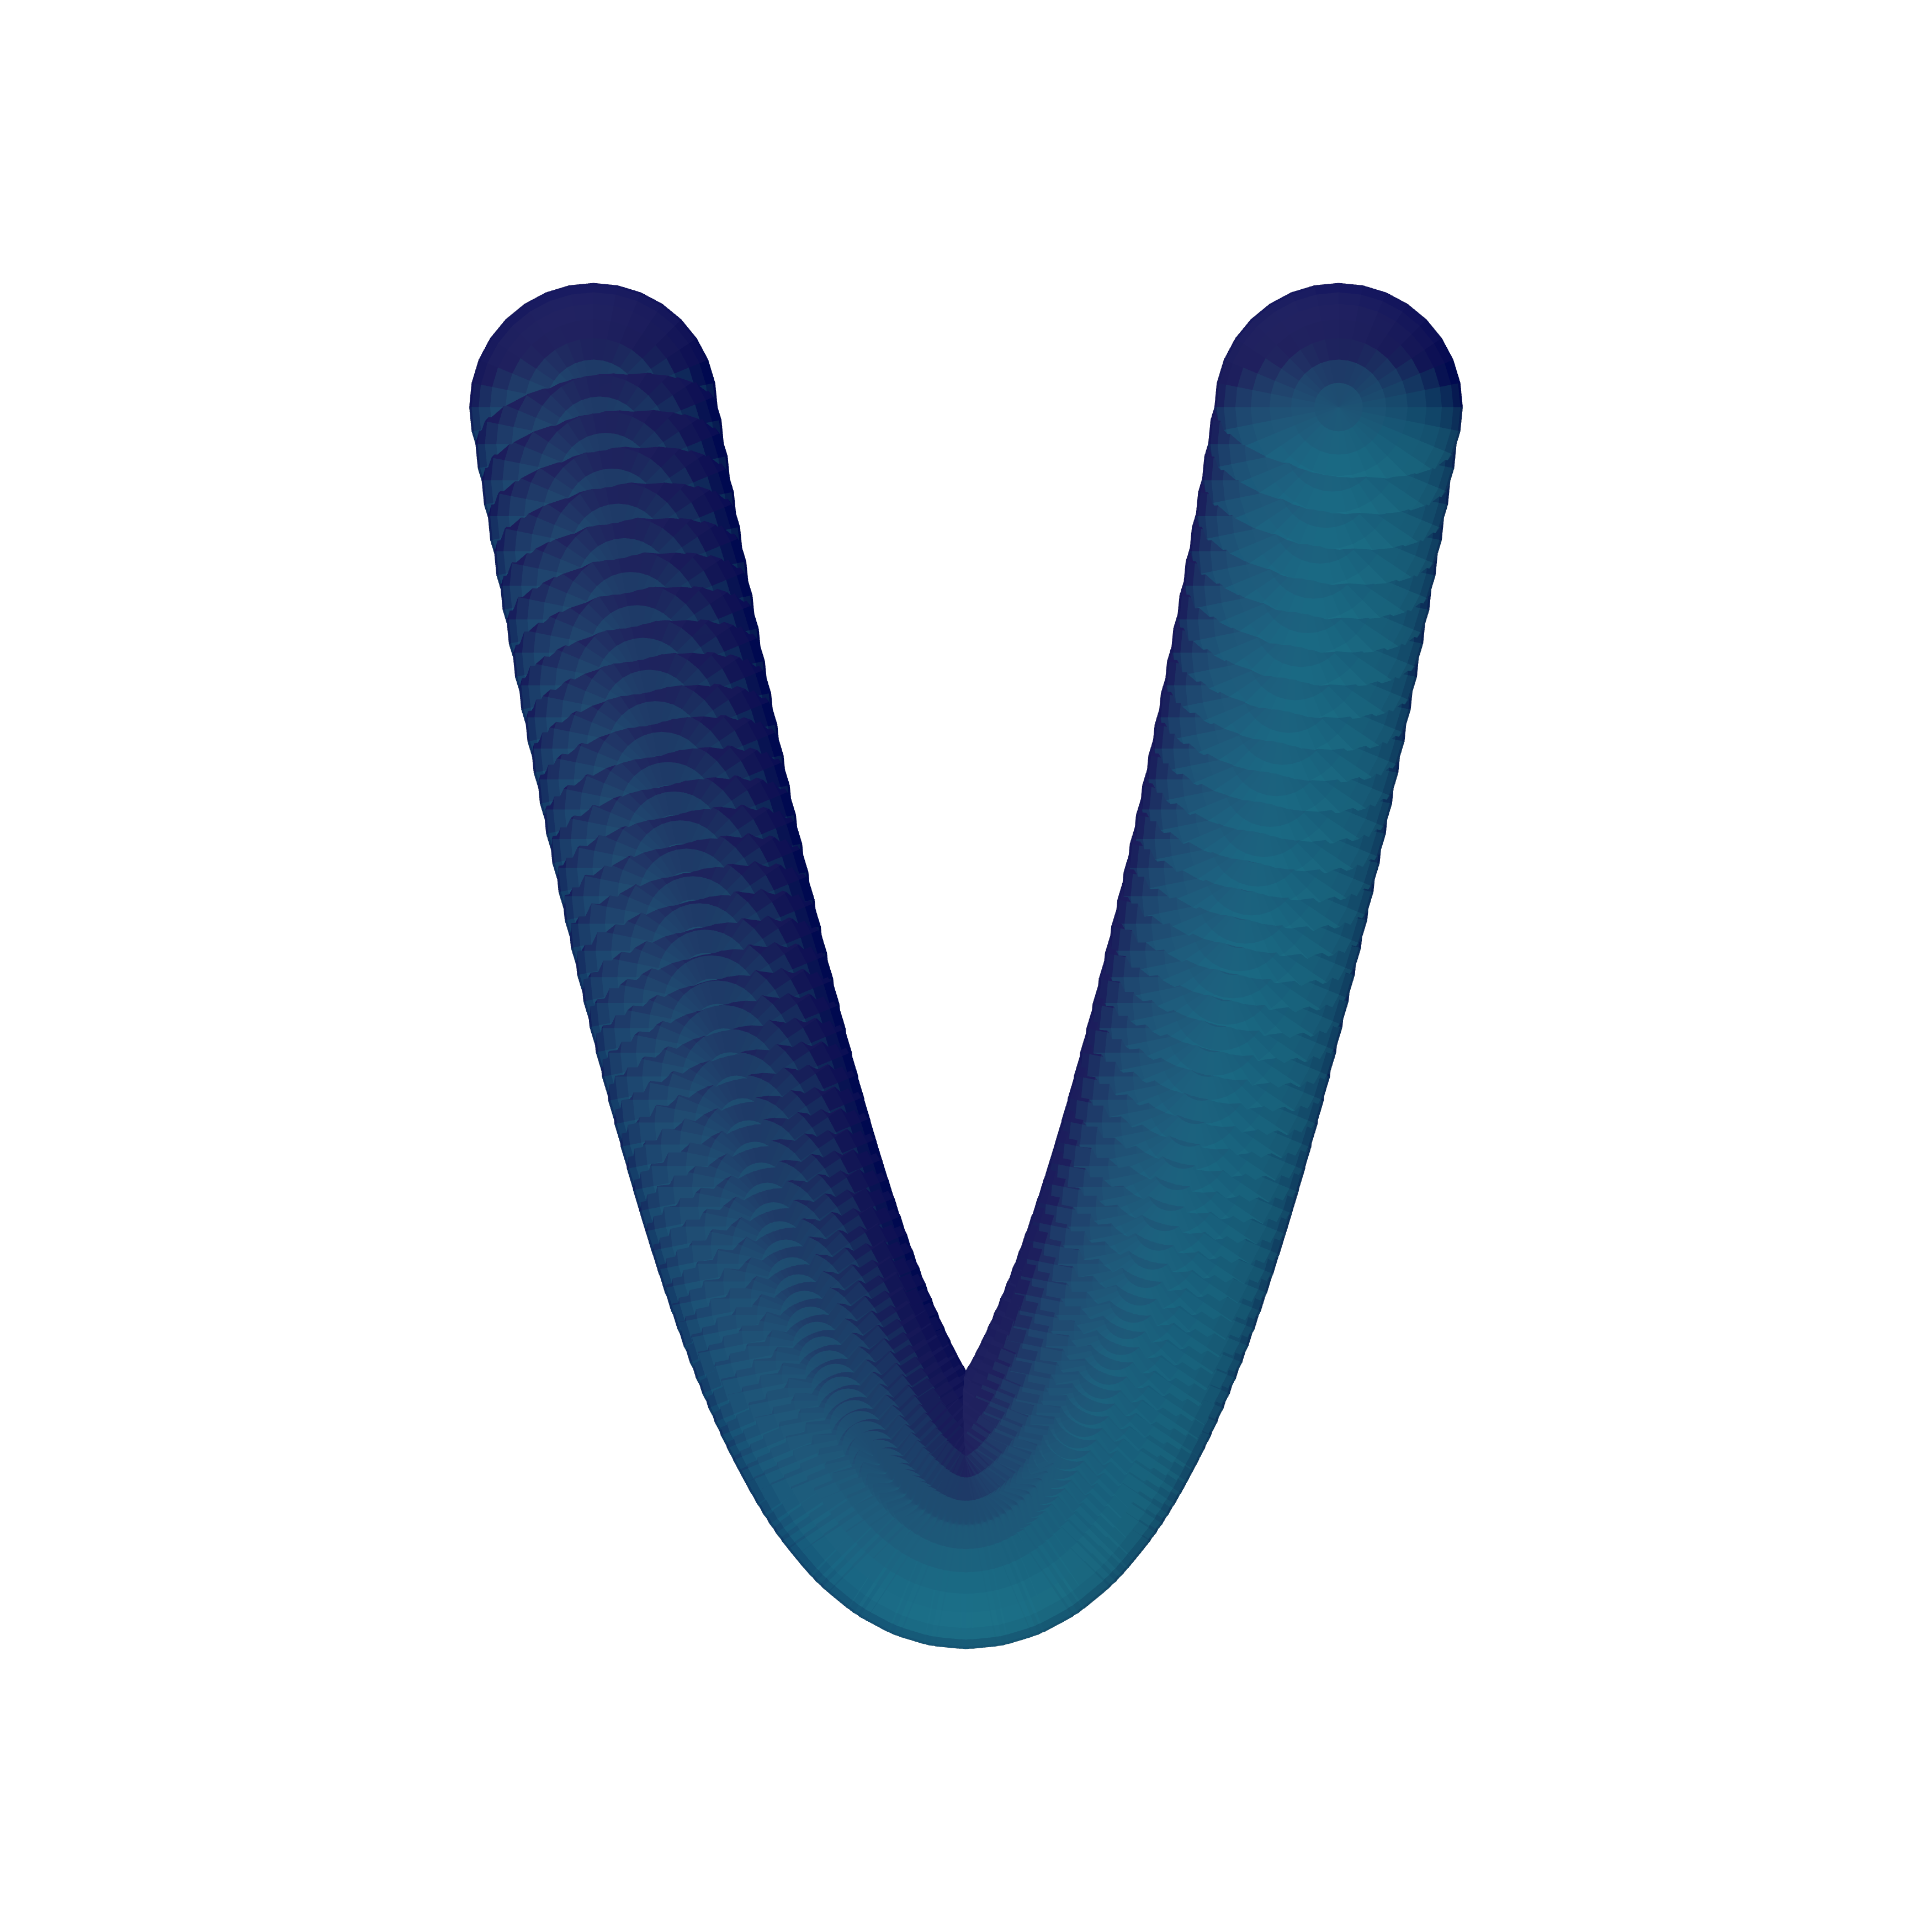
\includegraphics[width=\textwidth, trim=0mm 50mm 0mm 80mm, clip=true]{images/bienert_constant_radius_spheres.png}
        	\caption{Jednoparametrický systém sfér s~konštantným polomerom $r=1$.}
        \label{fig:plocha1}
    \end{subfigure}
    \begin{subfigure}[t]{0.49\textwidth}
        \centering
        
\includegraphics[width=\textwidth, trim=0mm 50mm 0mm 80mm, clip=true]{images/bienert_constant_radius_envelope.png}
		\caption{Obálka jednoparametrického systému sfér s~konštantným polomerom $r=1$.}
        \label{fig:plocha2}
    \end{subfigure}
    \hfill
    \begin{subfigure}[t]{0.49\textwidth}
        \centering
        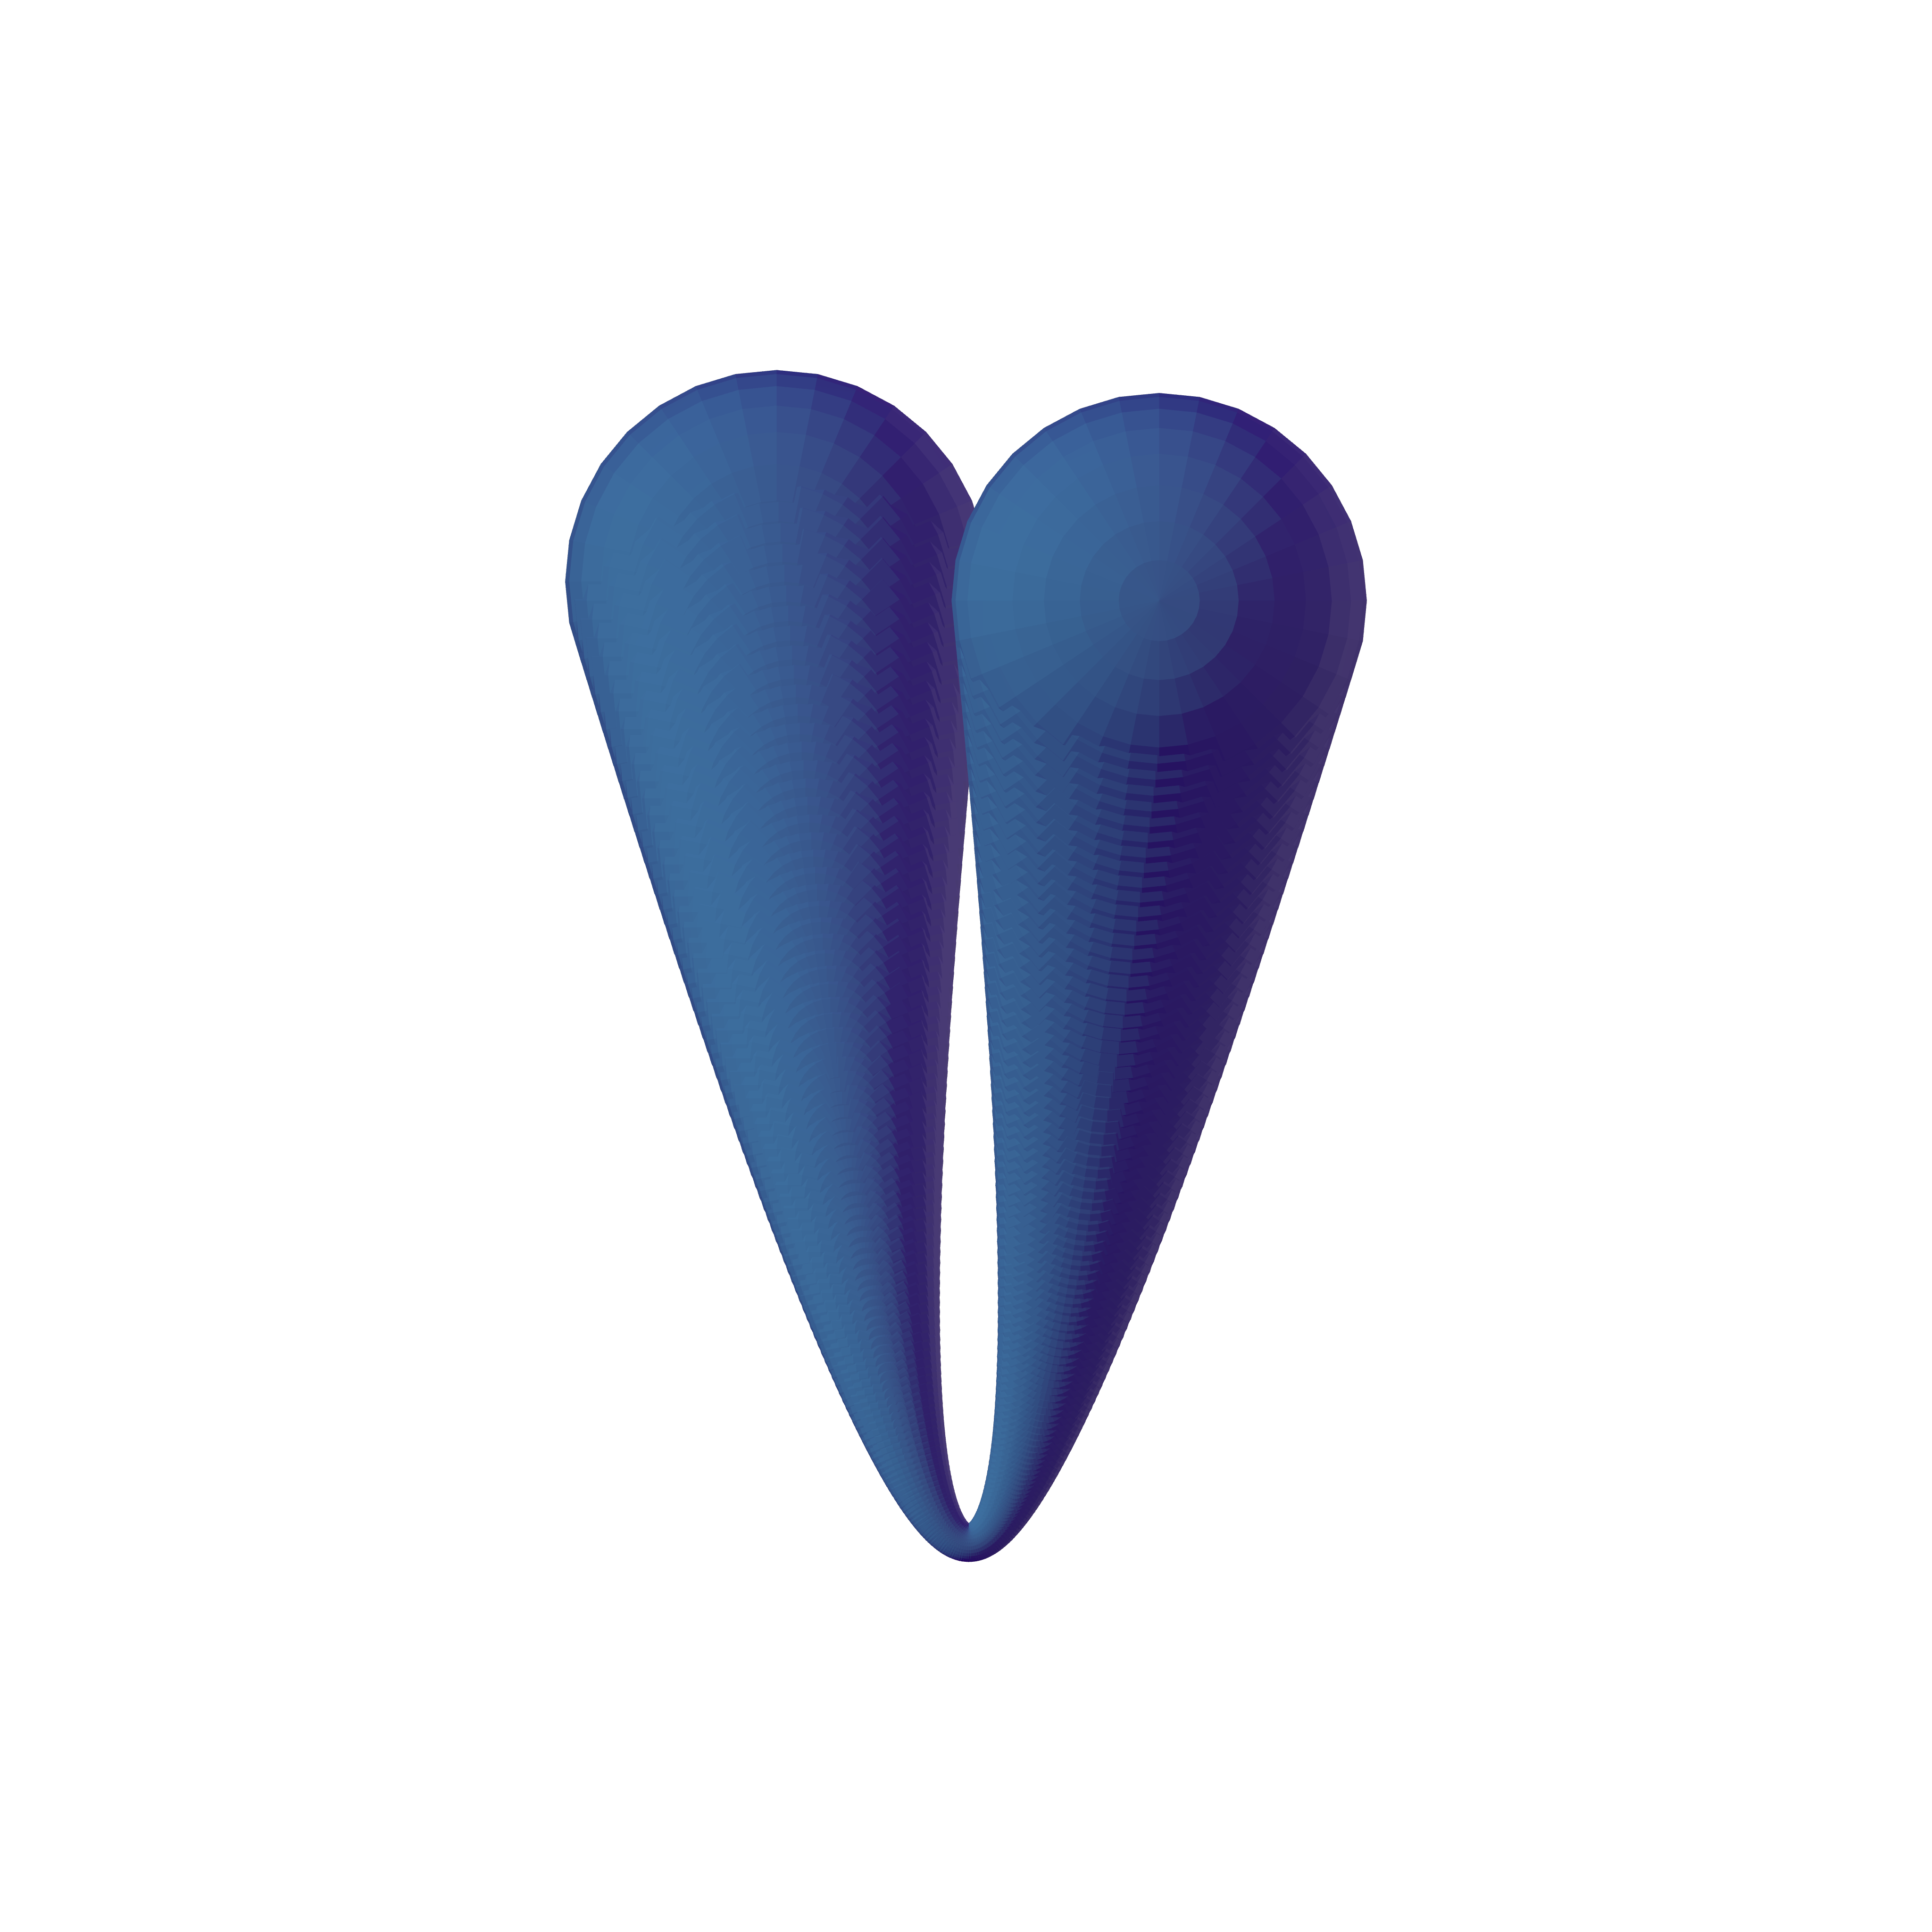
\includegraphics[width=\textwidth, trim=0mm 50mm 0mm 50mm, clip=true]{images/bienert_function_radius_spheres.png}
        	\caption{Jednoparametrický systém sfér s~funkciou polomeru $r=\frac{t^2}{5}-\frac{1}{2}$.}
        \label{fig:plocha3}
    \end{subfigure}
    \hfill
    \begin{subfigure}[t]{0.49\textwidth}
        \centering
        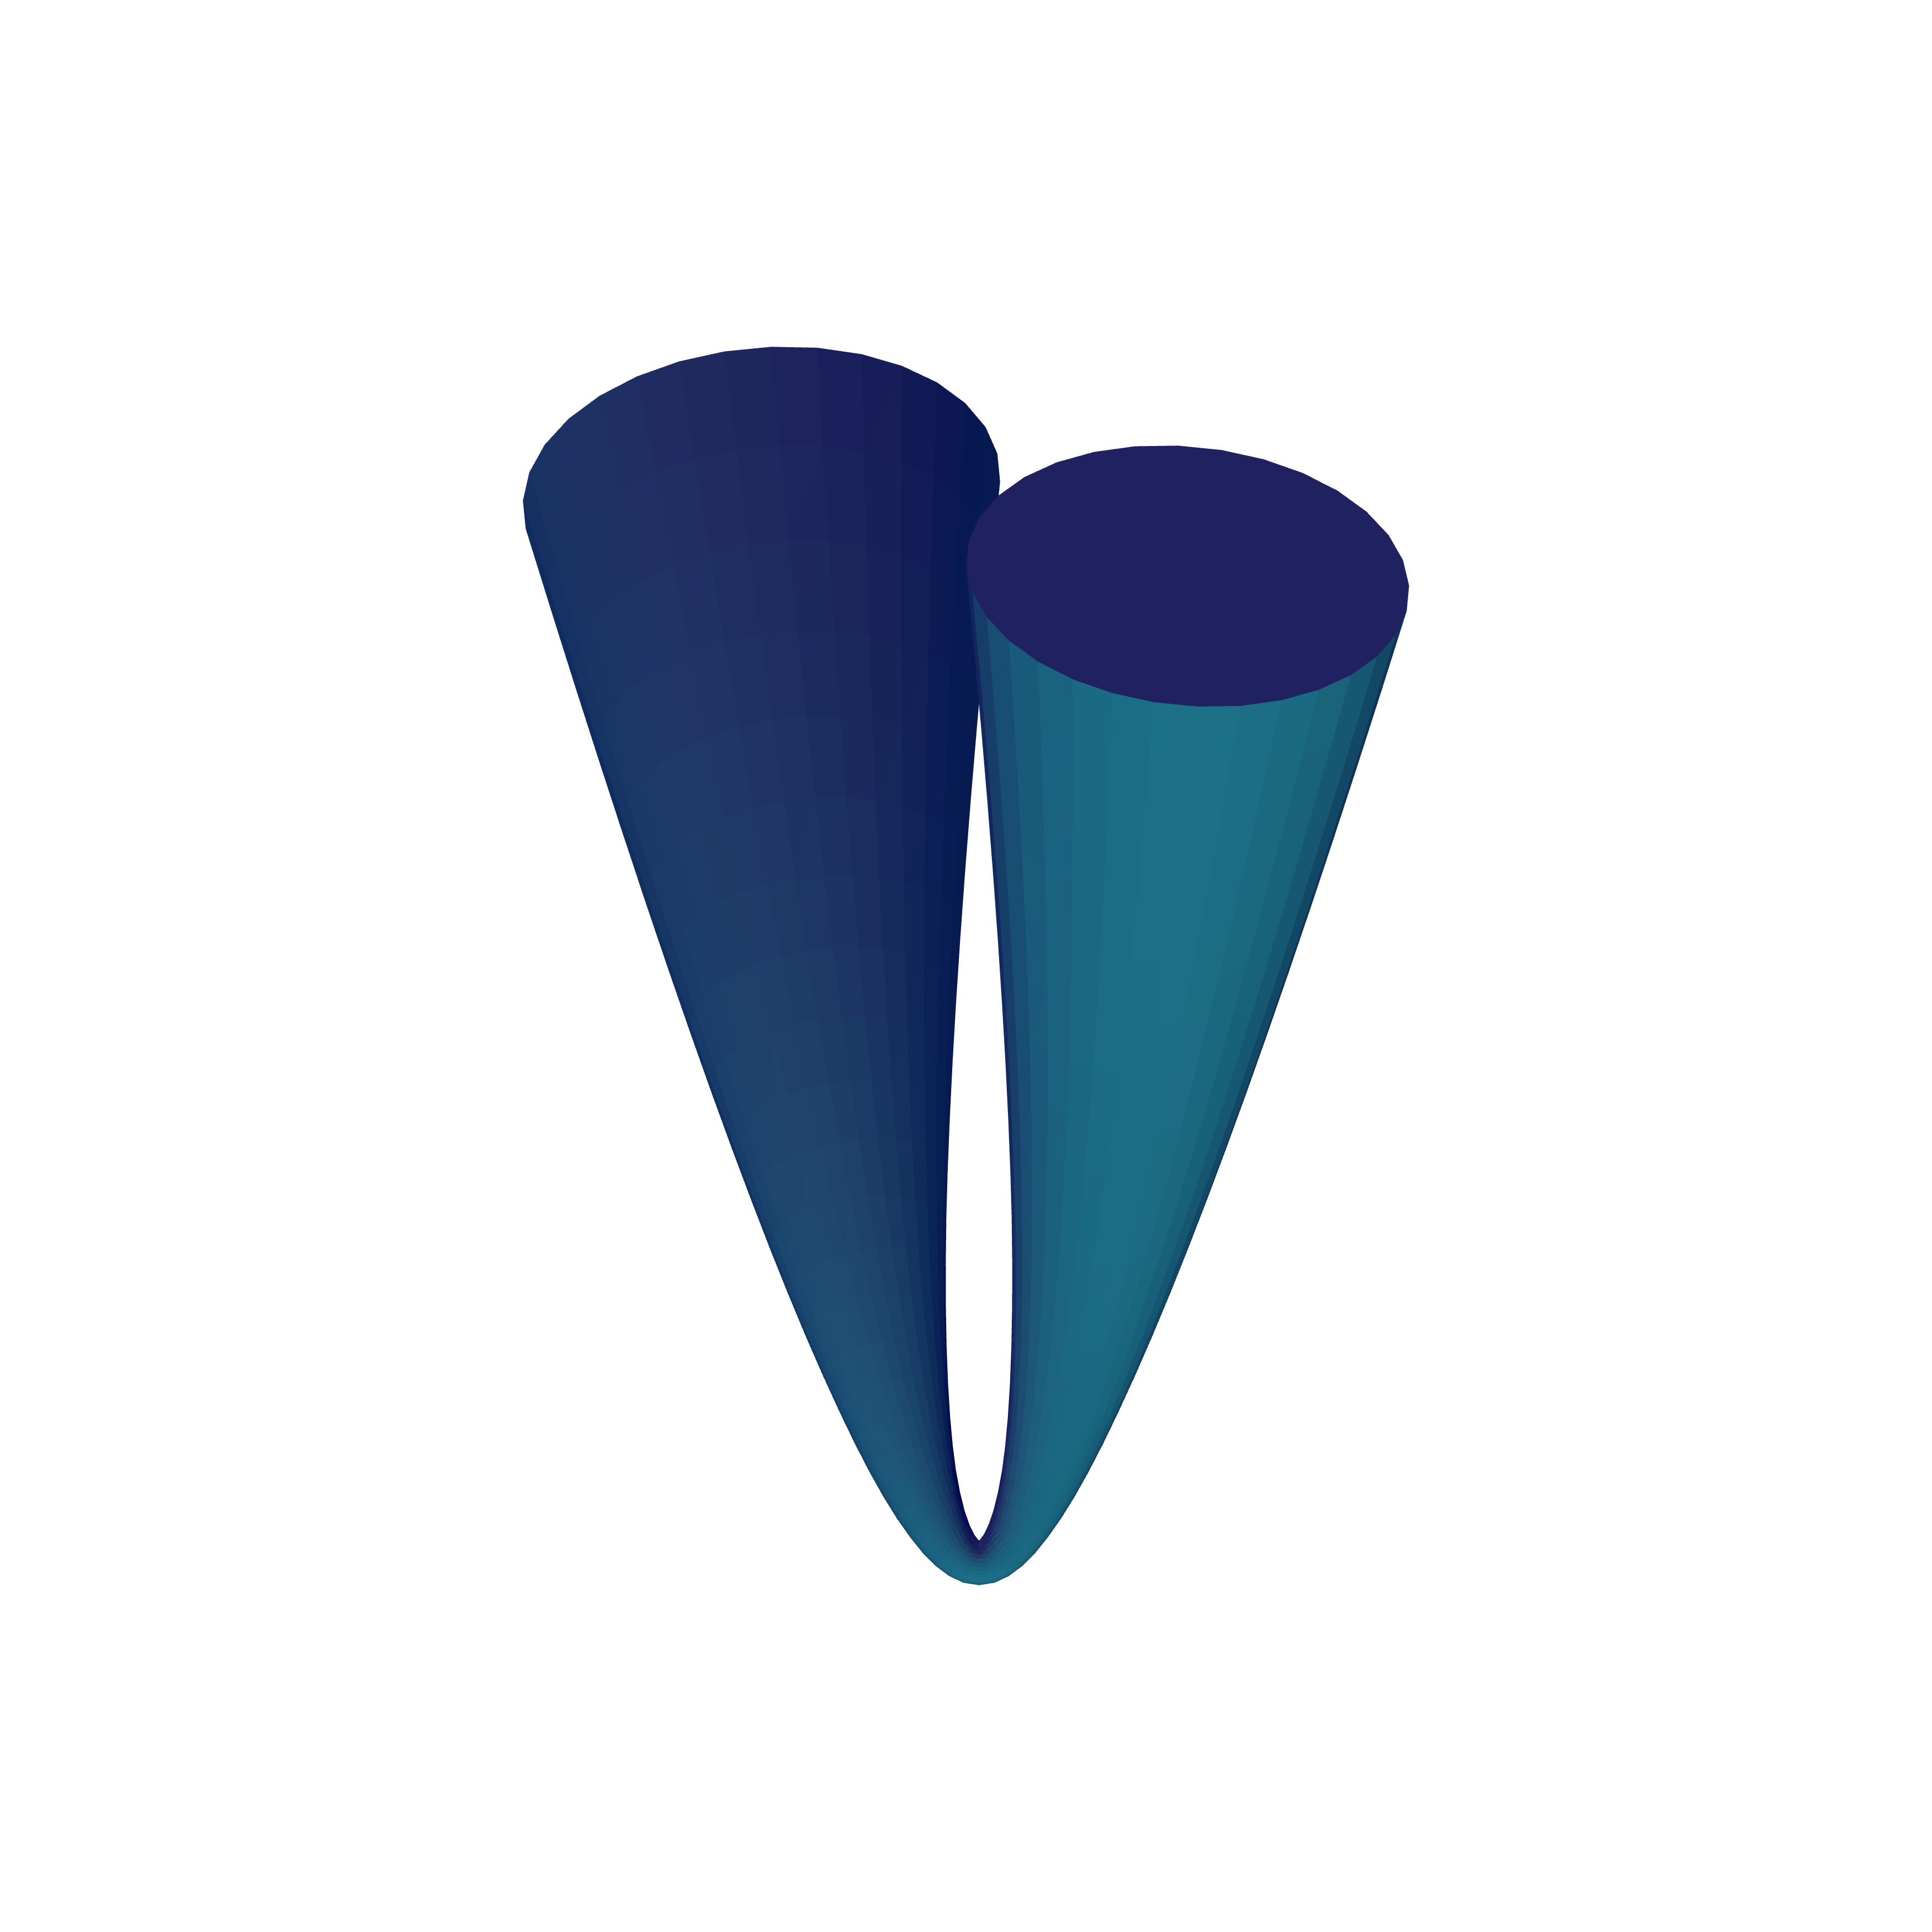
\includegraphics[width=\textwidth, trim=0mm 50mm 0mm 50mm, clip=true]{images/bienert_function_radius_envelope.png}
        	\caption{Obálka jednoparametrického systém sfér s~funkciou polomeru $r=\frac{t^2}{5}-\frac{1}{2}$.}
        \label{fig:plocha4}
    \end{subfigure}
    \begin{subfigure}[t]{0.49\textwidth}
        \centering
        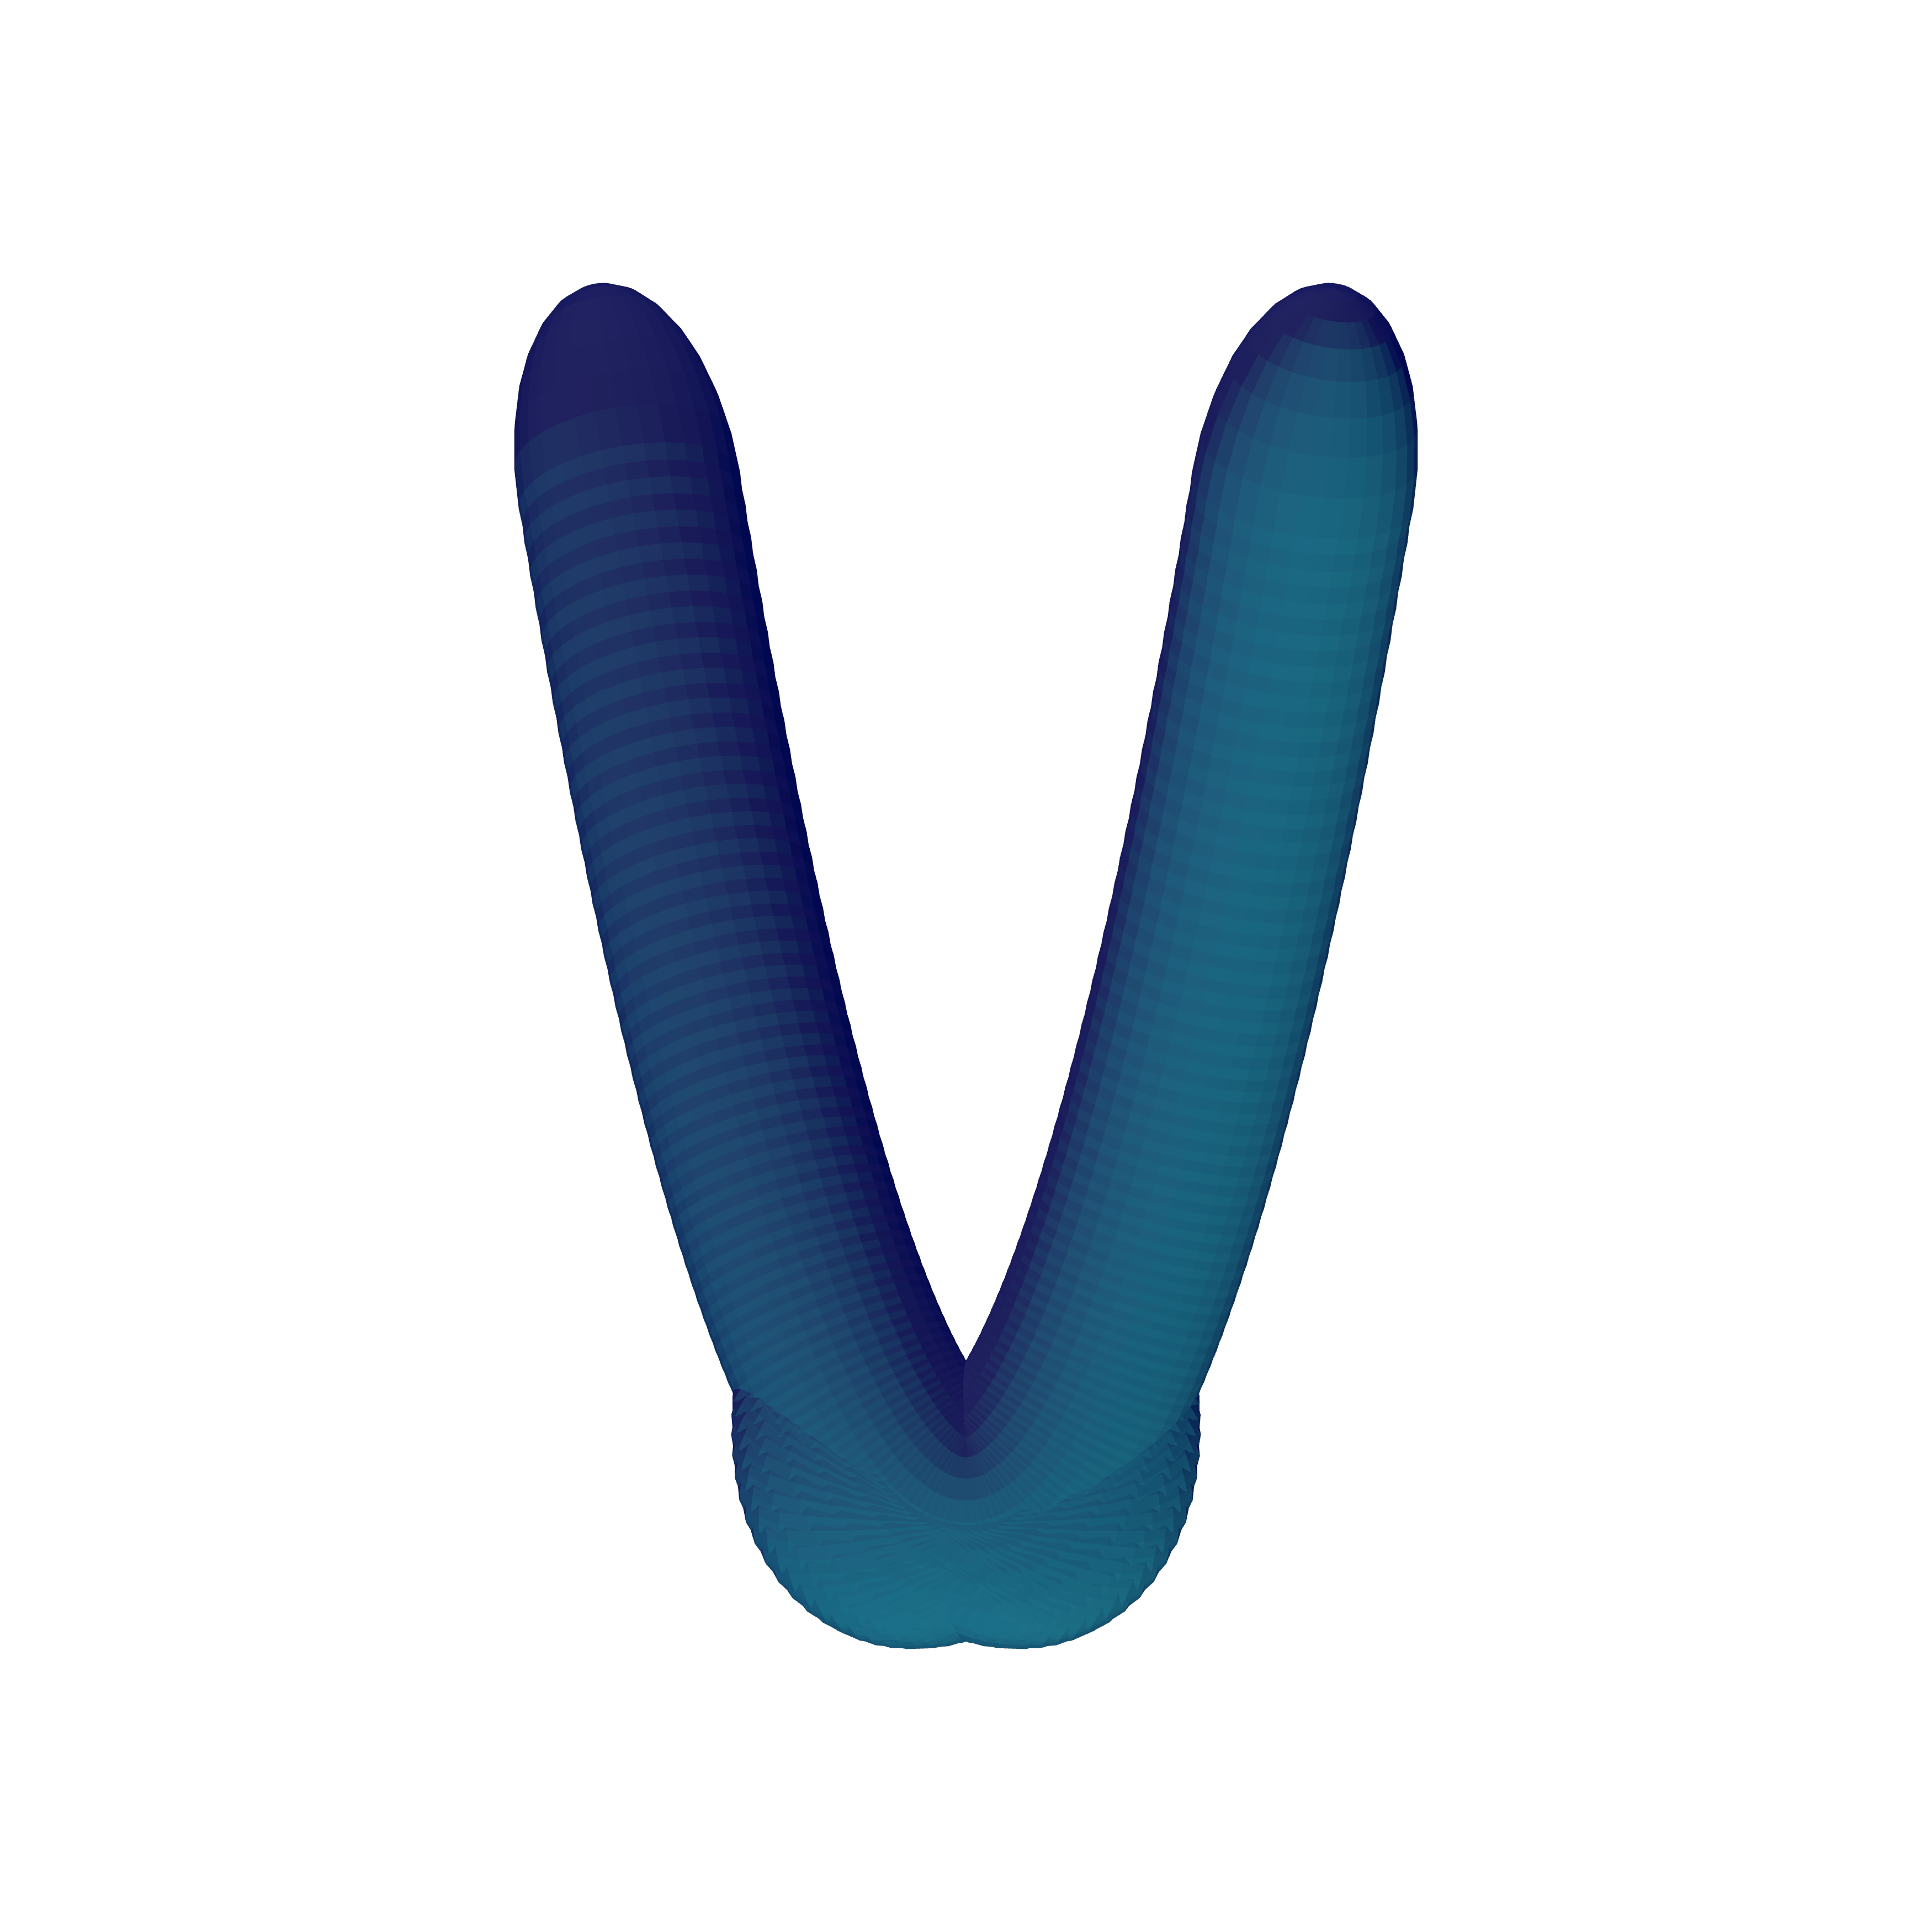
\includegraphics[width=\textwidth, trim=0mm 50mm 0mm 50mm, clip=true]{images/bienert_ellipsoids.png}
		\caption{Jednoparametrický systém elipsoidov so~škálovaním $a=2$ a $b=1$.}
        \label{fig:plocha5}
    \end{subfigure}
    \hfill
    \begin{subfigure}[t]{0.49\textwidth}
        \centering
        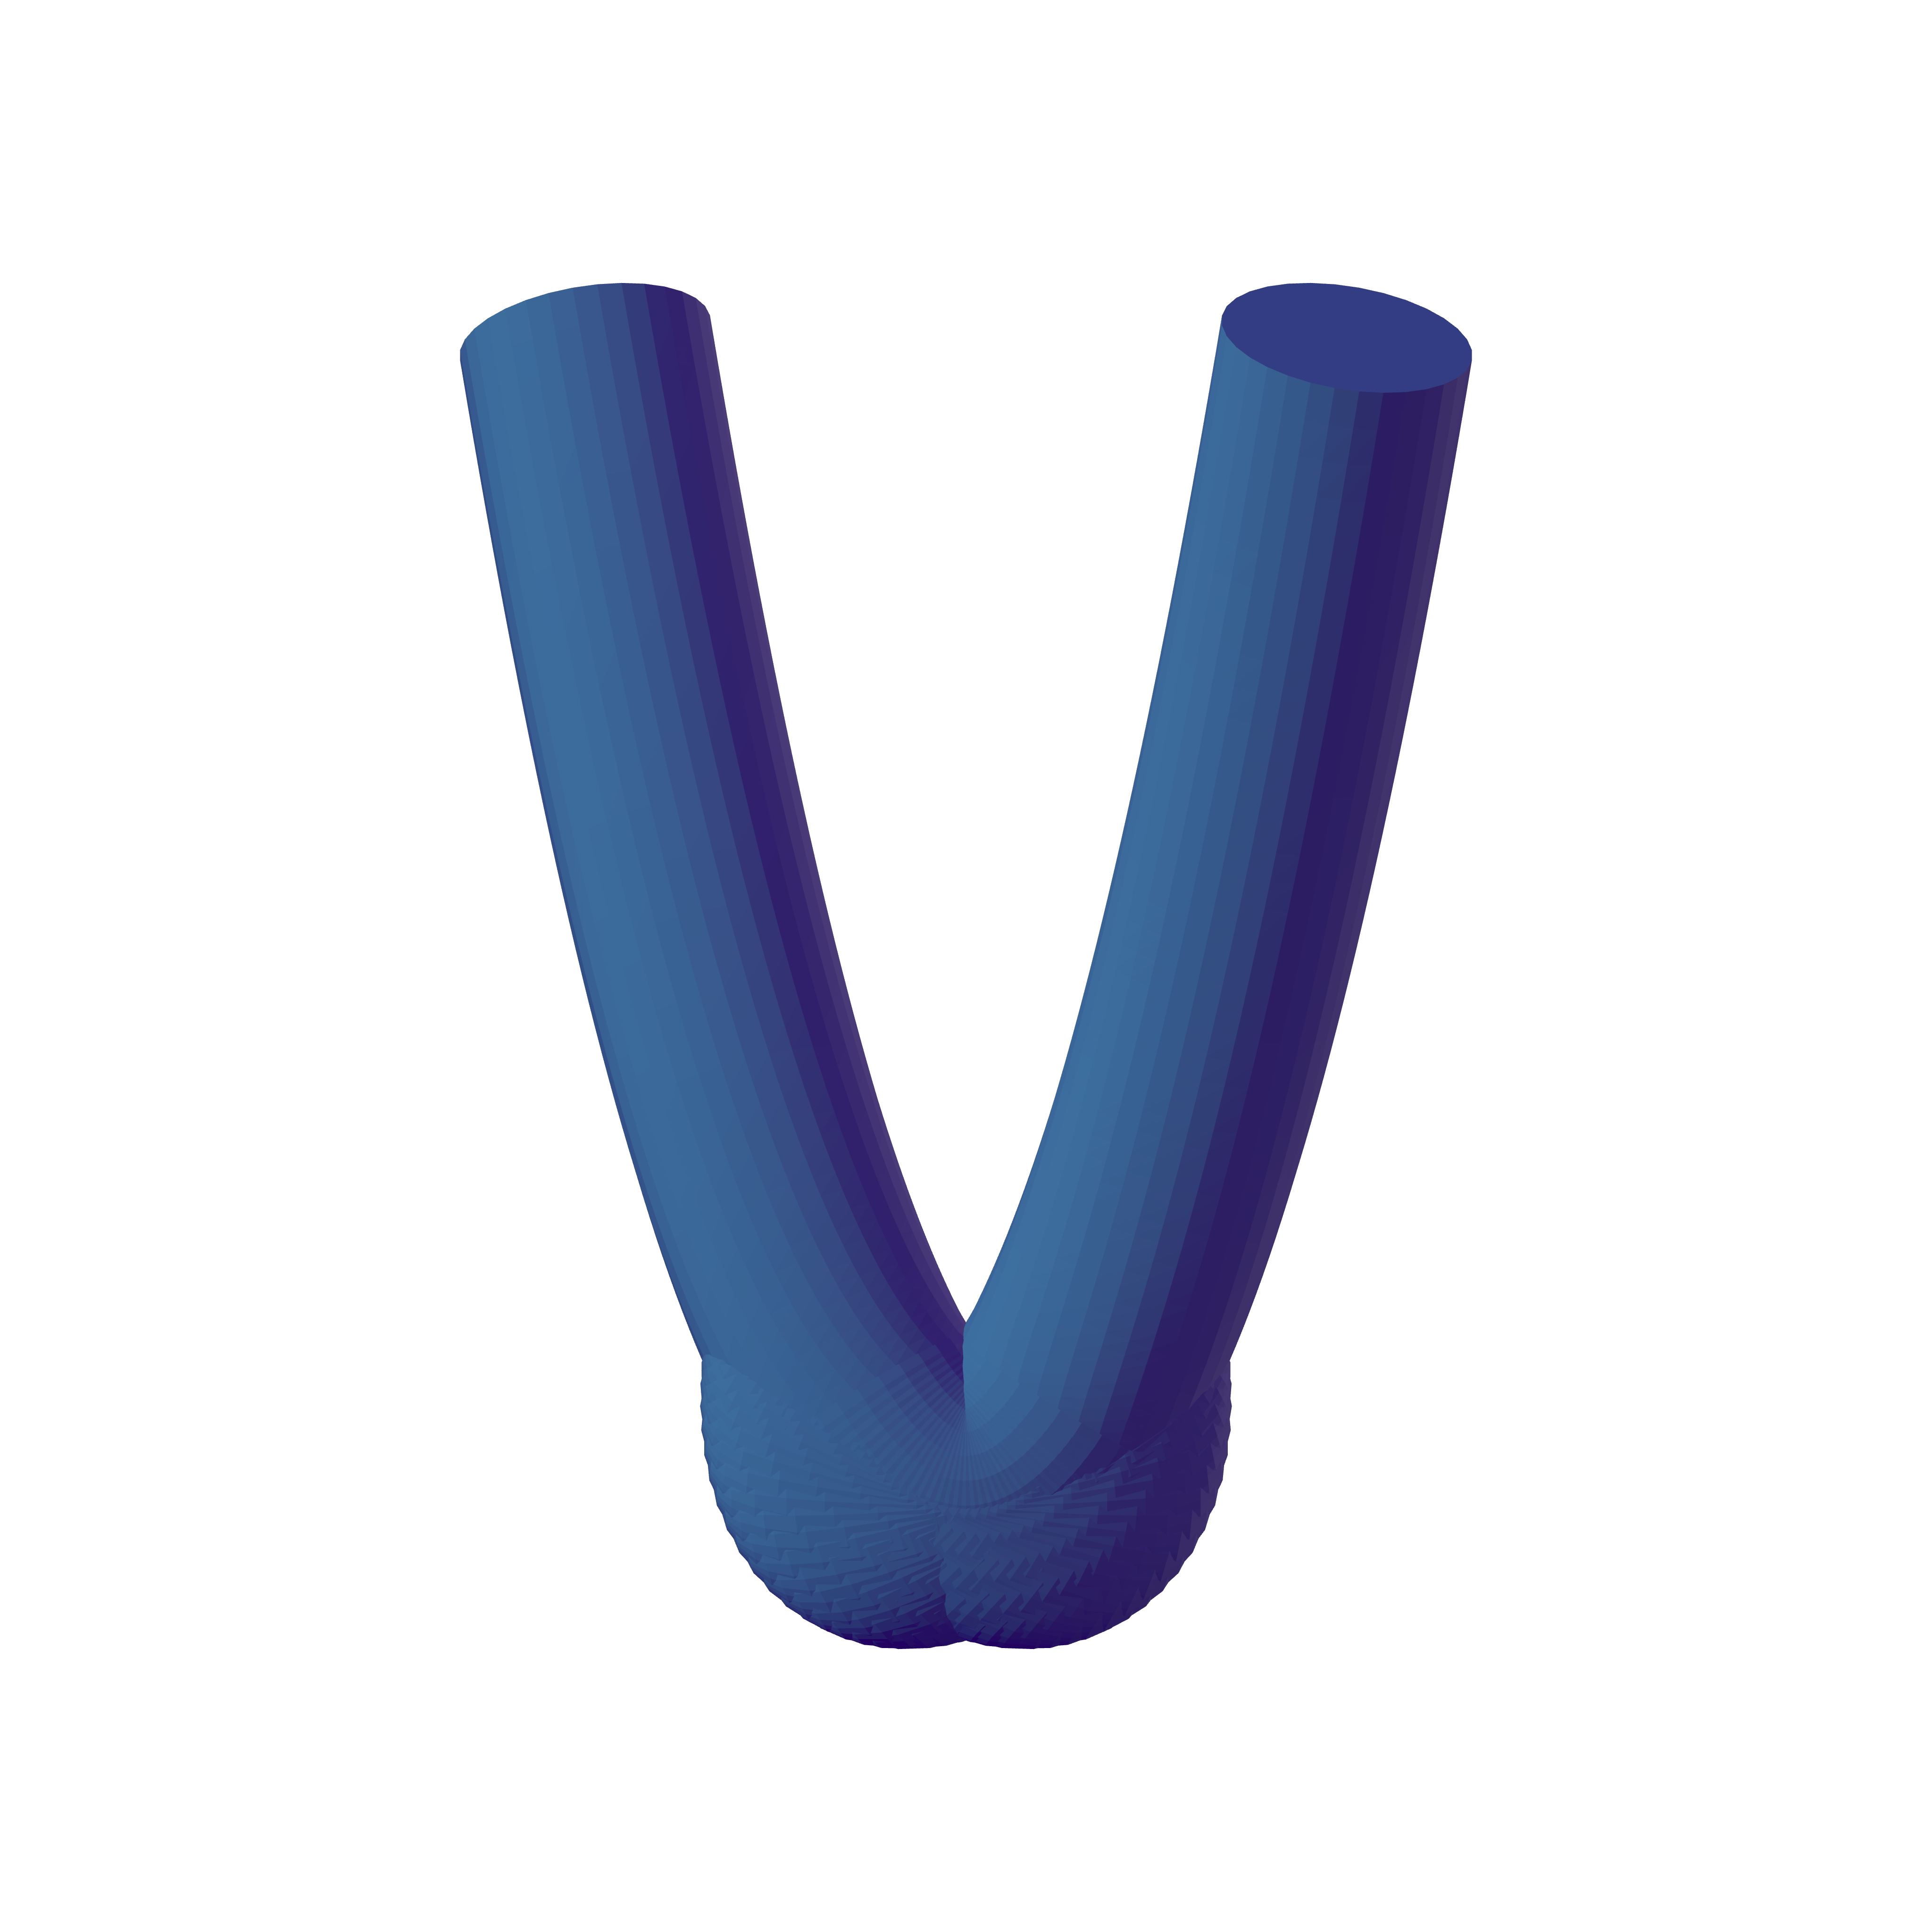
\includegraphics[width=\textwidth, trim=0mm 50mm 0mm 50mm, clip=true]{images/bienert_ellipsoids_envelope.png}
        	\caption{Obálka jednoparametrického systému elipsoidov so~škálovaním $a=2$ a $b=1$.}
        \label{fig:plocha6}
    \end{subfigure}
    	\caption[Jednoparametrické systémy a ich obálky ležiace na krivke Bienert.]{Jednoparametrické systémy a ich obálky ležiace na krivke s parametrizáciou  $m(t)=(t, t^2, \frac{t^3}{10}), \  t \in [-3, 3]$ a krokom $\Delta t = 0,05$.}
    \label{fig:katalogI}
\end{figure}
\begin{figure}[t!]
	\captionsetup{justification=centering}
	\captionsetup[subfigure]{justification=centering}
    \begin{subfigure}[t]{0.32\textwidth}
        \centering
        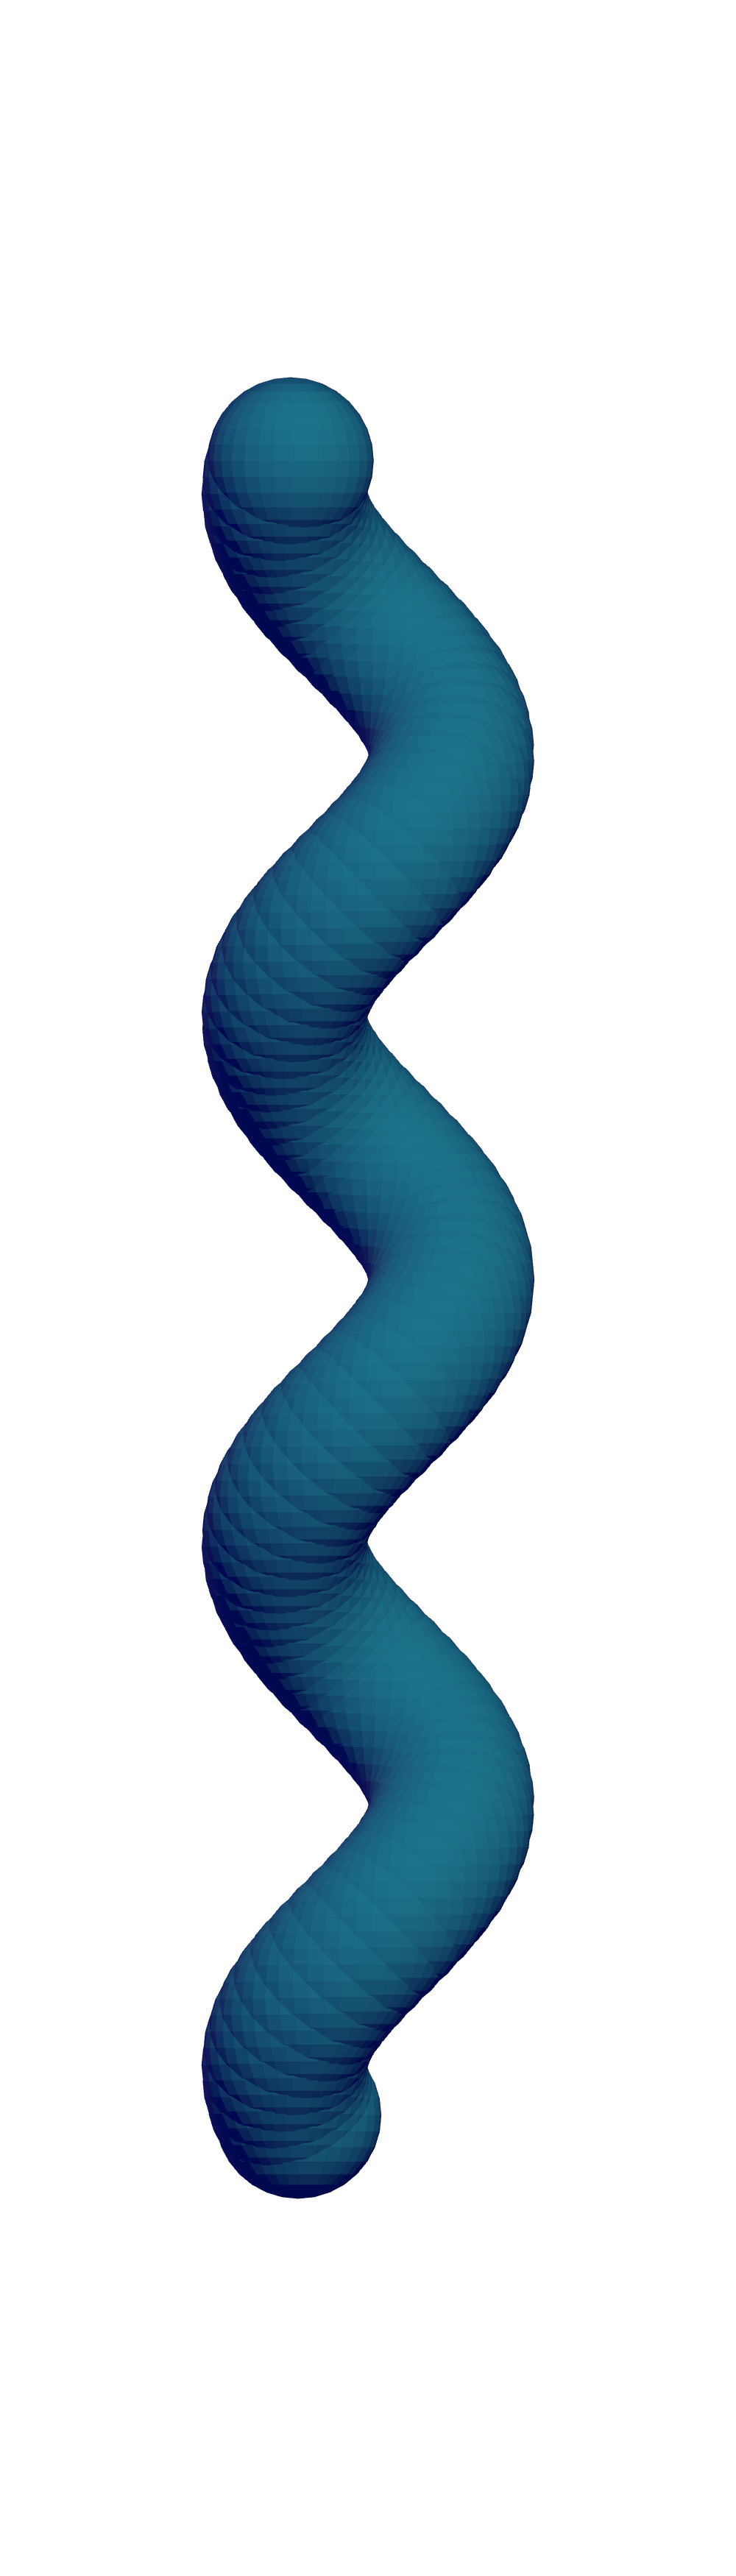
\includegraphics[width=0.45\textwidth, trim=0mm 80mm 0mm 80mm, clip=true]{images/helix_spheres.png}
		\caption{Jednoparametrický systém sfér s~konštantnou funkciou polomeru $r=1.$}
        \label{fig:plocha7}
    \end{subfigure}
    \hfill
    \begin{subfigure}[t]{0.32\textwidth}
        \centering
        
\includegraphics[width=0.45\textwidth, trim=0mm 80mm 0mm 80mm, clip=true]{images/helix_envelope.png}
        	\caption{Obálka systému sfér s~konštantnou funkciou polomeru $r=1$.}
        \label{fig:plocha8}
    \end{subfigure}
    \hfill
    \begin{subfigure}[t]{0.32\textwidth}
        \centering
        
\includegraphics[width=0.45\textwidth, trim=0mm 80mm 0mm 80mm, clip=true]{images/helix_ellipsoids.png}
        	\caption{Jednoparametrický systém elipsoidov so~škálovaním $a=2$ a $b=1$.}
        \label{fig:plocha9}
    \end{subfigure}
    	\caption[Jednoparametrické systémy a ich obálky ležiace na krivke skrutkovica.]{Jednoparametrické systémy a ich obálky ležiace na krivke s~parametrizáciou  $m(t)=(\cos t, \sin t, t), \  t \in [-10, 10]$ a krokom $\Delta t = 0,2$.}
    \label{fig:katalogII}
\end{figure}
\begin{figure}[h]
    \centering
    \captionsetup{justification=centering}
	\captionsetup[subfigure]{justification=centering}
    \begin{subfigure}[t]{0.49\textwidth}
        \centering
        
\includegraphics[width=0.82\textwidth, trim=0mm 100mm 0mm 50mm, clip=true]{images/heart_spheres.png}
        	\caption{Jednoparametrický systém sfér s~polomerom $r=1$.}
        \label{fig:plocha11}
    \end{subfigure}
    \hfill
    \begin{subfigure}[t]{0.49\textwidth}
        \centering
        
\includegraphics[width=0.82\textwidth, trim=0mm 100mm 0mm 50mm, clip=true]{images/heart_spheres_envelope.png}
        	\caption{Obálka jednoparametrického systému sfér s~polomerom $r=1$.}
        \label{fig:plocha12}
    \end{subfigure}
    \hfill
    \begin{subfigure}[t]{0.49\textwidth}
        \centering
        
\includegraphics[width=0.82\textwidth, trim=0mm 80mm 0mm 50mm, clip=true]{images/heart_ellipsoids.png}
        	\caption{Jednoparametrický systém elipsoidov so~škálovaním $a=3$ a $b=1$.}
        \label{fig:plocha13}
    \end{subfigure}
    \hfill
    \begin{subfigure}[t]{0.49\textwidth}
        \centering
        
\includegraphics[width=0.82\textwidth, trim=0mm 80mm 0mm 50mm, clip=true]{images/heart_ellipsoids_envelope.png}
        	\caption{Obálka jednoparametrického systému elipsoidov so~škálovaním $a=3$ a $b=1$.}
        \label{fig:plocha14}
    \end{subfigure}
    \caption[Jednoparametrické systémy a ich obálky ležiace na krivke srdce.]{Jednoparametrické systémy a ich obálky ležiace na krivke s~parametrizáciou $m(t)=(10\sin^{3}t, 8 \cos t-3\cos(2t) -\cos(3t)-\cos (4t), 0)$, $t \in [-\pi, \pi]$ a krokom $\Delta t = 0,05.$}
    \label{fig:katalogIII}
\end{figure}
\end{document}